% !TeX program = pdflatex
\documentclass[border=6pt]{standalone}
\usepackage{tikz}
\usetikzlibrary{arrows.meta, positioning, calc, fit, backgrounds}

\definecolor{MediumRed}{rgb}{0.925, 0.345, 0.345}
\definecolor{MediumGreen}{rgb}{0.37, 0.7, 0.66}
\definecolor{MediumBlue}{rgb}{0.015, 0.315, 0.45}
\definecolor{DarkBlue}{rgb}{0.05, 0.15, 0.35}

\begin{document}
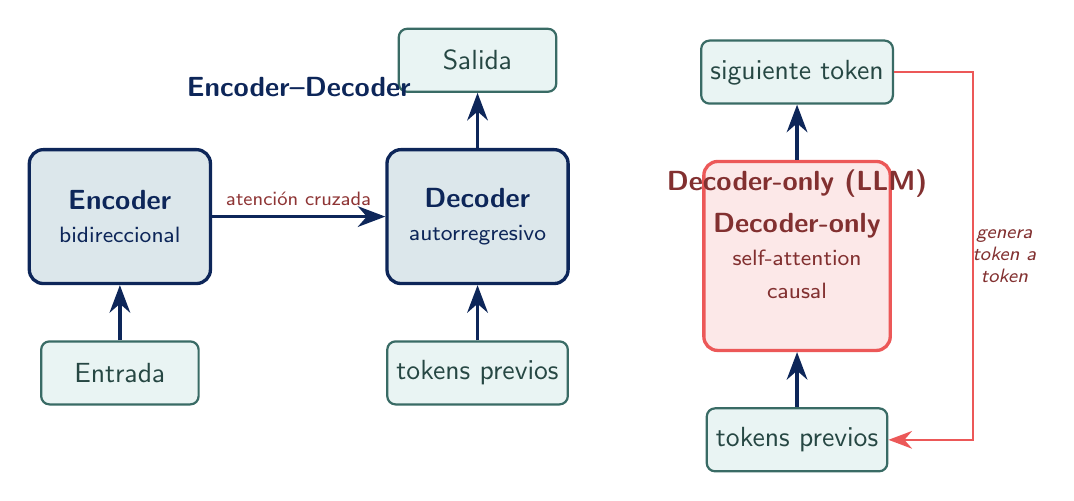
\begin{tikzpicture}[
    font=\sffamily,
    blk/.style={draw=DarkBlue, very thick, rounded corners=5pt, fill=MediumBlue!14,
        text=DarkBlue, align=center, minimum width=2.3cm, minimum height=1.7cm},
    io/.style={draw=MediumGreen!60!black, thick, rounded corners=3pt, fill=MediumGreen!14,
        text=MediumGreen!40!black, align=center, minimum width=2.0cm, minimum height=0.8cm},
    flow/.style={-{Stealth[length=3.5mm]}, line width=1.2pt, DarkBlue},
]

% ================= IZQUIERDA: encoder-decoder =================
\node[io] (ein) at (0,0) {Entrada};
\node[blk, above=0.7cm of ein] (enc) {\textbf{Encoder}\\\footnotesize bidireccional};
\node[blk, right=2.2cm of enc] (dec) {\textbf{Decoder}\\\footnotesize autorregresivo};
\node[io, below=0.7cm of dec] (dprev) {tokens previos};
\node[io, above=0.7cm of dec] (dout) {Salida};
\draw[flow] (ein)--(enc);
\draw[flow] (enc) -- node[above, font=\sffamily\scriptsize, text=MediumRed!60!black]
    {atención cruzada} (dec);
\draw[flow] (dprev)--(dec);
\draw[flow] (dec)--(dout);
\node[font=\sffamily\bfseries, text=DarkBlue] at ($(enc)!0.5!(dec)+(0,1.65)$) {Encoder--Decoder};

% ================= DERECHA: decoder-only =================
\begin{scope}[shift={(8.6,0)}]
    \node[io] (din) at (0,-0.85) {tokens previos};
    \node[blk, above=0.7cm of din, draw=MediumRed, fill=MediumRed!14,
          text=MediumRed!55!black, minimum height=2.4cm] (do) {\textbf{Decoder-only}\\\footnotesize self-attention\\\footnotesize causal};
    \node[io, above=0.7cm of do] (doout) {siguiente token};
    \draw[flow] (din)--(do);
    \draw[flow] (do)--(doout);
    % bucle autorregresivo
    \draw[-{Stealth[length=3mm]}, MediumRed, thick]
        (doout.east) -- ++(1.0,0) |- (din.east);
    \node[font=\sffamily\bfseries, text=MediumRed!55!black] at (0,2.4) {Decoder-only (LLM)};
    \node[font=\sffamily\scriptsize\itshape, text=MediumRed!55!black, align=center, right=0.9cm of do] {genera\\token a\\token};
\end{scope}

\end{tikzpicture}
\end{document}
